

Considere la matriz pentadiagonal $A= pentadiag_n(-1,-1,10,-1,-1)$, asuma que $n=10$ y $A=M+N+D$, con $D=diag(8,...,8) \in R^{10x10}$,  $A= pentadiag_n(-1,-1,1,0,0)$ y $N=M^t$. Para resolver el sistema de ecuaciones $Ax=b$, analice la convergencia de los siguientes metodos iterativos.
\begin{itemize}
    \item $(M+D)x^{k+1}=-Nx^k + b$ 
    \item $Dx^{k+1}=-(M+N)x^k + b$
    \item $(M+N)x^{k+1}=-Dx^k + b$
\end{itemize}

\textbf{Solución:}
\\
Sabemos que un método iterativo para resolver un sistema de ecuaciones de la forma:
$$Ax=b$$
es definido como:
$$x=Bx+b$$
Para comprobar la convergencia de un método iterativo se debe cumplir la condición:
$$\rho (B)<1$$ 
Ahora calculemos las matrices $M, D$ y $N$
    $$A=\begin{bmatrix}
    10&-1&-1&0&0&0&0&0&0&0\\
    -1&10&-1&-1&0&0&0&0&0&0\\
    -1&-1&10&-1&-1&0&0&0&0&0\\
    0&-1&-1&10&-1&-1&0&0&0&0\\
    0&0&-1&-1&10&-1&-1&0&0&0\\
    0&0&0&-1&-1&10&-1&-1&0&0\\
    0&0&0&0&-1&-1&10&-1&-1&0\\
    0&0&0&0&0&-1&-1&10&-1&-1\\
    0&0&0&0&0&0&-1&-1&10&-1\\
    0&0&0&0&0&0&0&-1&-1&10\\
    \end{bmatrix}$$
    
     $$M=\begin{bmatrix}
    1&0&0&0&0&0&0&0&0&0\\
    -1&1&0&0&0&0&0&0&0&0\\
    -1&-1&1&0&0&0&0&0&0&0\\
    0&-1&-1&1&0&0&0&0&0&0\\
    0&0&-1&-1&1&0&0&0&0&0\\
    0&0&0&-1&-1&1&0&0&0&0\\
    0&0&0&0&-1&-1&1&0&0&0\\
    0&0&0&0&0&-1&-1&1&0&0\\
    0&0&0&0&0&0&-1&-1&1&0\\
    0&0&0&0&0&0&0&-1&-1&1\\
    \end{bmatrix}$$
    $$D=\begin{bmatrix}
    8&0&0&0&0&0&0&0&0&0\\
    0&8&0&0&0&0&0&0&0&0\\
    0&0&8&0&0&0&0&0&0&0\\
    0&0&0&8&0&0&0&0&0&0\\
    0&0&0&0&8&0&0&0&0&0\\
    0&0&0&0&0&8&0&0&0&0\\
    0&0&0&0&0&0&8&0&0&0\\
    0&0&0&0&0&0&0&8&0&0\\
    0&0&0&0&0&0&0&0&8&0\\
    0&0&0&0&0&0&0&0&0&8\\
    \end{bmatrix}$$
    
    $$A=\begin{bmatrix}
    1&-1&-1&0&0&0&0&0&0&0\\
    0&1&-1&-1&0&0&0&0&0&0\\
    0&0&1&-1&-1&0&0&0&0&0\\
    0&0&0&1&-1&-1&0&0&0&0\\
    0&0&0&0&1&-1&-1&0&0&0\\
    0&0&0&0&0&1&-1&-1&0&0\\
    0&0&0&0&0&0&1&-1&-1&0\\
    0&0&0&0&0&0&0&1&-1&-1\\
    0&0&0&0&0&0&0&0&1&-1\\
    0&0&0&0&0&0&0&0&0&1\\
    \end{bmatrix}$$
\begin{itemize}
    \item $(M+D)x^{k+1}=-Nx^k + b$ \\
    Primero despejamos para obtener $B$.
    $$x^{k+1}=-(M+D)^{-1}Nx^k + -(M+D)^{-1}b$$
    $$B=-(M+D)^{-1}N$$
    Calculando la matriz B con octave obtenemos:
   \begin{figure}[H]
                \centering
                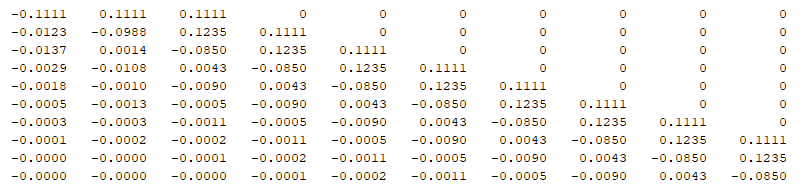
\includegraphics[width=1.1\textwidth]{matrix_images/b1.PNG}
                \caption{Matriz B}
        \end{figure}
    Ahora calculemos el radio espectral de la matriz $B$. Para ello calcularemos los eigenvalores de $B$:
    $$eig(B)=\begin{bmatrix}
    -0.0214 + 0.0911i\\
  -0.0214 - 0.0911i\\
  -0.0586 + 0.0764i\\
  -0.0586 - 0.0764i\\
  -0.0937 + 0.0417i\\
  -0.0937 - 0.0417i\\
  -0.1441 + 0.0167i\\
  -0.1441 - 0.0167i\\
  -0.1436 + 0.0000i\\
  -0.1111 + 0.0000i\\
    \end{bmatrix}
    $$
    El radio espectral de $B$ es el mayor eigenvalor en valor absoluto de $B$.
    $$\rho (B) = 0.1450 <1$$
    Por lo que concluimos que el método CONVERGE.
    
    \item $Dx^{k+1}=-(M+N)x^k + b$ 
    \begin{itemize}
        \item Despejamos para obtener B:
        $$x^{k+1}=-D^{-1}(M+N)x^k + D^{-1}b$$ 
        $$B=-D^{-1}(M+N)$$
    \item Calculamos la matriz B:
    \begin{figure}[H]
                \centering
                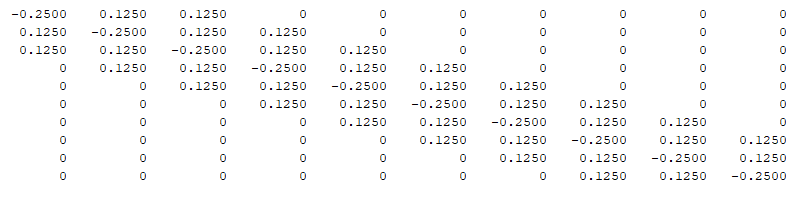
\includegraphics[width=1.1\textwidth]{matrix_images/b2.PNG}
                \caption{Matriz B}
        \end{figure}
    \item Calculamos el radio espectral de $B$:
     Para ello calcularemos los eigenvalores de $B$:
    $$eig(B)=\begin{bmatrix}
              -0.5000\\
           -0.5000\\
           -0.4222\\
           -0.4096\\
           -0.3327\\
           -0.2842\\
           -0.2500\\
           -0.0874\\
            0.0814\\
            0.2048\\
    \end{bmatrix}
    $$
    El radio espectral de $B$ es el mayor eigenvalor en valor absoluto de $B$.
    $$\rho (B) = 0.5000<1$$
    \item Entonces concluimos que el método CONVERGE.
    \end{itemize}
    
    
    
    
    \item $(M+N)x^{k+1}=-Dx^k + b$
    \begin{itemize}
        \item Despejamos para obtener B:
        $$x^{k+1}=-(M+N)^{-1}Dx^k + b$$ 
        $$B=-(M+N)^{-1}D$$
    \item Calculamos la matriz B:
    \begin{figure}[H]
                \centering
                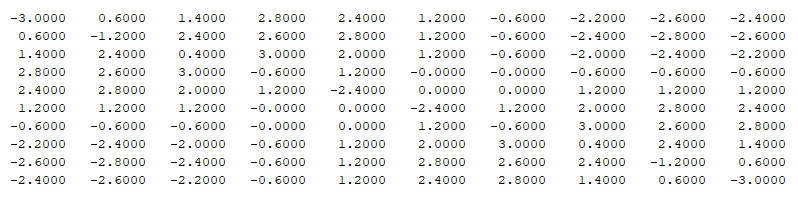
\includegraphics[width=1.1\textwidth]{matrix_images/b3.PNG}
                \caption{Matriz B}
        \end{figure}
    \item Calculamos el radio espectral de $B$:
    Para ello calcularemos los eigenvalores de $B$:
    $$eig(B)=\begin{bmatrix}
            -11.4356\\
           -4.0000\\
           -3.5182\\
           -3.0054\\
           -2.4411\\
           -2.3688\\
           -2.0000\\
           -2.0000\\
            4.8821\\
   12.2870
    \end{bmatrix}
    $$
    El radio espectral de $B$ es el mayor eigenvalor en valor absoluto de $B$.
    $$\rho (B) = 12.2870>1$$
    \item Entonces concluimos que el metodo NO CONVERGE.
    \end{itemize}
\end{itemize}